%\documentclass{article}
\documentclass[journal,12pt,twocolumn]{IEEEtran}

% Language setting
% Replace `english' with e.g. `spanish' to change the document language
\usepackage[english]{babel}

% Set page size and margins
% Replace `letterpaper' with `a4paper' for UK/EU standard size
%%\usepackage[letterpaper,top=2cm,bottom=2cm,left=3cm,right=3cm,marginparwidth=1.75cm]{geometry}

% Useful packages
\usepackage[utf8]{inputenc}
%\usepackage{enumitem}
\usepackage{multicol}
\usepackage{ragged2e}
\usepackage{amsmath}
\usepackage{amssymb}
\usepackage{graphicx}
\usepackage{array}
\usepackage{blindtext}
%\usepackage[paperwidth=10cm]{geometry}
\usepackage{tkz-euclide}
%\usepackage{tikz}
\usetikzlibrary{
  circuits.logic,
  circuits.logic.US,
  positioning
}

\usepackage[colorlinks=true, allcolors=blue]{hyperref}

\title{Line Assignment}
\author{Navya Valmeekam}
\begin{document}
\maketitle
\tableofcontents
\section{Problem}
In Fig. 1, ABCD is a parallelogram and BC is produced to a point Q such that AD = CQ. If AQ intersect DC at P, show that ar (BPC) = ar (DPQ).
[Hint : Join AC.]
\begin{tikzpicture}[scale=0.90]
    %initialisation
    \tkzInit[xmin=0,xmax=6,ymin=-2.8,ymax=2.8] 
    \tkzClip[space=1] 
    %definitions
    \tkzDefPoint(0,0){D} 
    \tkzDefPoint(1,2.8){A} 
    \tkzDefPoint(6,2.8){B} 
    \tkzDefPoint(5,0){C}
    \tkzDefPoint(2.5,0){P} 
    \tkzDefPoint(4,-2.8){Q}  
    \tkzDrawPolygon(A,B,C,D)
    %\tkzDrawPolygon(A,C,Q,D)
    \tkzDrawSegments(B,P)
    \tkzDrawSegments(A,Q)
    \tkzDrawSegments(D,Q)
    \tkzDrawSegments(C,Q)
    \tkzLabelPoints[above right](C)
     \tkzLabelPoints[above](P,Q)
    \tkzLabelPoints[above left](A,B,D)
\end{tikzpicture}
%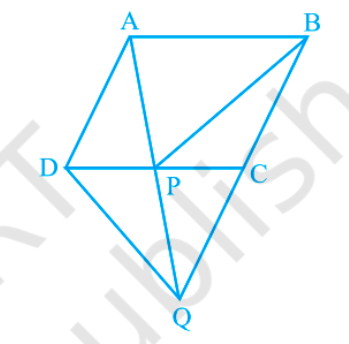
\includegraphics[scale=0.5]{image.png}
\begin{center}
Figure 1
\end{center}
%\end{abstract}
\section{Solution}
\justify
\textbf{Construction: Join AC}\\
\textbf{Theoretical Proof:}\\
\textbf{To Prove:}
ar($\Delta$ BPC) = ar($\Delta$ DPQ)\\
Since ABCD is a paralellogram, $ AD \: || \: BC $\\
and BC is extended to point Q\\
\begin{enumerate}
$\therefore$ $ AD \: || \: CQ $\\ and AD=CQ  (given)\\
\end{enumerate}
\textbf{A quadrilateral is said to be paralellogram if a pair of its opposite sides are parallel and equal}\\
\begin{enumerate}
$\therefore$ ACQD is a paralellogram\\
\end{enumerate}
By the theorem,\\
\textbf{Theorem:}
\textbf{Two triangles on the same base and between same parallels are equal in area}\\
\begin{enumerate}
ar($\Delta$ BPC) = ar($\Delta$ APC)......(1)\\
\end{enumerate}
In $\Delta$ APC and $\Delta$ DPQ,\\
\begin{enumerate}
$\angle$ PAC = $\angle$ PQD [Alternate interior angles are equal]\\ 
AC=QD [Opposite sides of a paralellogram are equal]\\
$\angle$ ACP = $\angle$ PDQ [Alternate interior angles are equal]\\
\end{enumerate}
By ASA rule,$\Delta$ APC and $\Delta$ DPQ are congruent\\
\begin{enumerate}
\item $\therefore$ ar($\Delta$ APC)=ar($\Delta$ DPQ)......(2) [Since congruent triangles have equal area]\\
\end{enumerate}
\textbf{From 1 and 2 ar($\Delta$ BPC)=ar($\Delta$ DPQ)}\\
hence proved\\
\justify
\textbf{To Prove:}
ar($\Delta$ BPC) = ar($\Delta$ DPQ)
\begin{flushleft}
Given ABCD is a paralellogram, and BC is produced to point Q such that AD=CQ. AQ intersect DC at P.\\
We need to prove that ar(BPC)=ar(DPQ)\\
Let,\hfill \\
\centering{A-B=$\vec{p1}$\hfill\\
           D-C=$\vec{s1}$\hfill\\
           A-D=$\vec{p2}$\hfill\\
           B-C=$\vec{s2}$\hfill}\\
\justify
\vspace{0.1cm}
By paralellogram property\\
\begin{enumerate}
$\lVert{p1}\rVert$ =$\lVert{s1}\rVert$ \&\& $\lVert{p2}\rVert$ =$\lVert{s2}\rVert$ \hspace{1.2cm}[1]\\
\end{enumerate}
\vspace{3cm}
Since P lies on DC,\\
\begin{enumerate}
DP=PC=k x DC\\
DP=PC=k($\vec{s1}$)\\
\end{enumerate}
Area of triangle BPC \\
\begin{enumerate}
=1/2 x [PC x BC] \\
=1/2 x [k($\vec{s1}$) x $\vec{s2}$] \\
= 1/2 x [k($\vec{p1}$) x ($\vec{p2}$)] (from [1])\\ 
\end{enumerate}
\textbf{Area of triangle BPC}\\
\vspace{0.1cm}
\textbf{=1/2 x [k($\vec{p1}$) x ($\vec{p2}$)]  \hspace{2.5cm}[2]}\\
\vspace{0.1cm}
Given that BC is extended to Q so,\\ 
\begin{enumerate}
$ AD \: || \: CQ $\\ and AD=CQ(given)\\ So, ACQD is a parallelogram \\
\end{enumerate}
\vspace{0.1cm}
AC=DQ. [Since opposite sides of a paralellogram are equal]
 \hspace{4.5cm} [3] \\
\vspace{0.1cm}
In triangle ABC,\\ 
\begin{enumerate}
AC=AB+BC\\    AC=(A-B)+(B-C)\\    AC=$\vec{p1}$ + $\vec{s2}$\\
 AC=$\vec{p1}$ + $\vec{p2}$ (from [1])\\
 From [3]\\ AC=DQ=$\vec{p1}$ + $\vec{p2}$ \hspace{2.5cm}[4]\\
\end{enumerate} 
Area of a triangle DPQ\\
\begin{enumerate}
=1/2 x [DP x DQ]\\
=1/2 x [k($\vec{s1}$) x ($\vec{p1}$ + $\vec{p2}$)] (from [4])\\ 
=1/2 x [k($\vec{p1}$) x ($\vec{p1}$ + $\vec{p2}$)]\\ 
=1/2 x [k($\vec{p1}$) x ($\vec{p1}$) + k($\vec{p1}$) x ($\vec{p2}$)]\\ 
=1/2 x [k($\vec{p1}$) x $\vec{p2}$)]\\
\end{enumerate}
\textbf{Area of triangle DPQ}\\
\vspace{0.1cm}
\textbf{=1/2 x [k($\vec{p1}$) x $\vec{p2}$)]  \hspace{2.5cm} [5]}\\
\vspace{0.1cm}
\textbf{from [2] and [5]}\\
\vspace{0.1cm}
\textbf{ar(BPC)=ar(DPQ)}\\
\vspace{0.1cm}
hence proved\\
%%\hspace{-1cm}By paralellogram property\\
%%\hspace{1cm}$\lVert{p1}\rVert$ =$\lVert{s1}\rVert$ \&\& $\lVert{p2}\rVert$ =$\lVert{s2}\rVert$ \hspace{1cm}[1]\\
%%\hspace{-2cm}Since P lies on DC,\\
%%                      DP=PC=k x DC\\
%%                      DP=PC=k($\vec{s1}$)\\
%%\hspace{-1cm}Area of triangle BPC \\
%%=1/2 x [PC x BC] \\
%%=1/2 x [k($\vec{s1}$) x $\vec{s2}$] \\
%%= 1/2 x [k($\vec{p1}$) x ($\vec{p2}$)] (from [1])\\ 
%%\textbf{Area of triangle BPC}\\
%%\textbf{=1/2 x [k($\vec{p1}$) x ($\vec{p2}$)]   [2]}\\
%%Given that BC is extended to Q so, $$ AD \: || \: CQ $$ and AD=CQ(given)\\
%%So, ACQD is a parallelogram \\
%% Therefore AC=DQ. [Since opposite sides of a paralellogram are equal] [3] \\
%% In triangle ABC,\\ AC=AB+BC\\
%%                  AC=(A-B)+(B-C)\\
%%                  AC=$\vec{p1}$ + $\vec{s2}$\\
%%                  AC=$\vec{p1}$ + $\vec{p2}$ (from [1])\\
%% From [3]\\ AC=DQ=$\vec{p1}$ + $\vec{p2}$ [4]\\ 
%%\hspace{1cm}Area of a triangle DPQ\\
%%=1/2 x [DP x DQ]\\
%%=1/2 x [k($\vec{s1}$) x ($\vec{p1}$ + $\vec{p2}$)] (from [4])\\ 
%%=1/2 x [k($\vec{p1}$) x ($\vec{p1}$ + $\vec{p2}$)]\\ 
%%=1/2 x [k($\vec{p1}$) x ($\vec{p1}$) + k($\vec{p1}$) x ($\vec{p2}$)]\\ 
%=1/2 x [k($\vec{p1}$) x $\vec{p2}$)]\\
%\textbf{Area of triangle DPQ}\\
%\textbf{=1/2 x [k($\vec{p1}$) x $\vec{p2}$)]   [5]}\\
%\textbf{from [2] and [5]}\\
%\textbf{ar(BPC)=ar(DPQ)}\\
%\textbf{hence proved}\\

\newpage
\textbf{Input parameters for this construction}
\begin{center}
\begin{tabular}{|c|c|c|}
\hline
\textbf{Symbol}&{Value}&{Description}\\
\hline
r0&5&DC\\
\hline
r1,r2&3,2.8&DA\\
\hline
r3,r4&4,173&CQ\\
\hline
r5,r6&10,3.4&CB\\
\hline
${\theta}_1$& 2$\pi/5$&$ \angle $ADC\\ 
\hline
${\theta}_2$& $\pi/200$&$ \angle $QDC\\ 
\hline
${\theta}_3$& 2$\pi/3.45$&$ \angle $BDC\\ 
\hline 
\end{tabular}
\end{center}

\section{Construction}
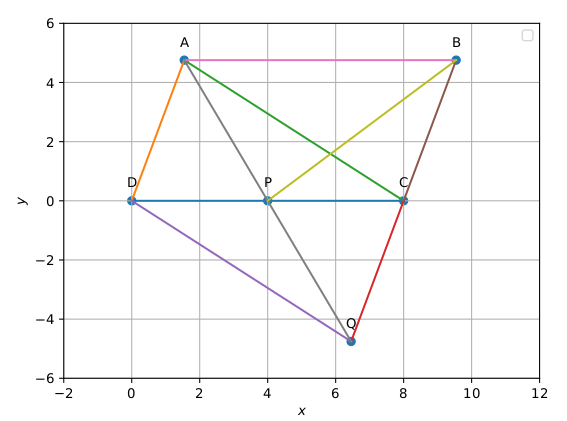
\includegraphics[scale=0.4]{construction.png}
\begin{center}
Figure of Construction
\end{center}
\end{flushleft}
\end{document}
